\documentclass[12pt,a4paper]{article}

% ============================================================================
% Packages
% ============================================================================
\usepackage[utf8]{inputenc}
\usepackage[T1]{fontenc}
\usepackage{amsmath,amssymb}
\usepackage{graphicx}
\usepackage[margin=2.5cm]{geometry}
\usepackage{natbib}  % For citation management
\usepackage{hyperref}
\usepackage{lineno}
\linenumbers

% ============================================================================
% Document Settings
% ============================================================================
\bibliographystyle{agsm}  % Harvard style, or use 'plainnat', 'apalike', etc.
% Other common styles: abbrvnat, unsrtnat, plainnat

\title{Shifting Balance of Thermal and Haline Forcing in Southern Ocean Dense Water Formation Across Glacial-Interglacial Cycles: A Water Mass Transformation Analysis}

\author{Xiaoxu Shi$^{1}$, Gerrit Lohmann$^{1,2}$, and Christian Stepanek$^{1}$ \\
\\
\small $^1$Alfred Wegener Institute, Helmholtz Centre for Polar and Marine Research, Bremerhaven, Germany \\
\small $^2$MARUM -- Center for Marine Environmental Sciences, University of Bremen, Bremen, Germany}

% Abbreviations used in this manuscript:
% DJF - December-January-February (austral summer)
% JJA - June-July-August (austral winter)
% LGM - Last Glacial Maximum
% LIG - Last Interglacial
% MH - Mid-Holocene
% MIS3 - Marine Isotope Stage 3
% MLD - Mixed Layer Depth
% PI - Preindustrial
% SAM - Southern Annular Mode
% SSS - Sea Surface Salinity
% SST - Sea Surface Temperature
% WMT - Water Mass Transformation

\date{\today}

% ============================================================================
% Document Begin
% ============================================================================
\begin{document}

\maketitle

% ============================================================================
% Abstract
% ============================================================================
\begin{abstract}
The Southern Ocean dense water formation is a key component of the global overturning circulation,  driving abyssal ventilation and regulating heat and carbon storage on centennial to millennial timescales. However, understanding how surface buoyancy forcing controls this formation across different climate states remains a fundamental challenge. Here, we analyze water mass transformation (WMT) in the AWI-ESM coupled model across five paleoclimate scenarios, i.e., preindustrial (PI), mid-Holocene (MH), Last Interglacial (LIG), Last Glacial Maximum (LGM), and Marine Isotope Stage 3 (MIS3). By systematically decomposing  surface buoyancy fluxes into thermal (longwave, shortwave, sensible, and latent heat) and haline (sea ice and precipitation-evaporation-runoff) components,  we identify a fundamental regime shift in forcing mechanisms. Specifically, interglacial WMT is thermally dominated, with heat fluxes driving 70–85\% of dense water formation. Conversely, glacial states exhibit haline-dominated forcing, where expanded sea ice governs transformation through the competing effects of adiabatic insulation and enhanced brine rejection. Superimposed on these mean states, we further evaluate the impact of atmospheric variability. Composite analysis reveals that the Southern Annular Mode (SAM) modulates WMT rates by 15–20\% across all climate states. During positive SAM phases, dense water formation is intensified via enhanced heat loss over open ocean and amplified brine rejection within coastal areas. Reflecting the shift in ventilation efficiency, our simulations show that deep ocean ventilation ages increase by about 1,500 years during glacial periods, with marked regional heterogeneity. These results highlight the non-linear state-dependence of surface forcing, offering a mechanistic framework for interpreting past Southern Ocean circulation changes.




\noindent\textbf{Keywords:} Southern Ocean, water mass transformation, paleoclimate, surface buoyancy flux,
sea ice, ventilation age
\end{abstract}

% ============================================================================
% Introduction
% ============================================================================
\section{Introduction}


\subsection{The Southern Ocean and global climate}

The Southern Ocean plays an important role in Earth's climate system. It serves as the primary region where deep waters return to the surface through wind-driven upwelling and where surface waters are transformed into dense water masses that ventilate the global abyssal ocean \citep{Marshall2012, Talley2013}. This region is characterized by intense air-sea interaction, extensive seasonal sea ice coverage, and strong meridional density gradients that drive both the upper and lower cells of the global meridional overturning circulation (MOC) \citep{Speer2000, Lumpkin2007}. Through this overturning circulation, the Southern Ocean regulates the global capacity to store heat and carbon \citep{Marinov2006, Gray2024}. Therefore, understanding the physical processes behind dense water formation in the Southern Ocean is crucial for predicting how the climate system will respond to future changes.


Surface buoyancy fluxes fundamentally control the transformation of water masses in density space \citep{Walin1982, Speer1992}. These fluxes consist of heat exchange with the atmosphere as well as freshwater fluxes caused by precipitation, evaporation, river runoff, and sea ice processes. In the Southern Ocean, these surface buoyancy fluxes exhibit pronounced spatial and seasonal variability. Specifically, intense wintertime cooling drives surface densification in open water regions, whereas sea ice formation and melting produce strong haline forcing through brine rejection and freshwater release \citep{Abernathey2016, Pellichero2018}. Observational evidence suggests that freshwater fluxes, particularly those associated with sea ice thermodynamics, may dominate in ice-covered regions \citep{Pellichero2018, Bailey2023}. However, quantifying the relative contribution of thermal versus haline forcing to dense water formation across the entire Southern Ocean still remains a topic of active research. 

The role of the Southern Ocean in the global carbon cycle is equally important. As the primary pathway for deep water ventilation, this region regulates carbon exchange between the deep ocean reservoir and the atmosphere \citep{Marinov2006, Gray2024}. The efficiency of this carbon sequestration process depends critically on the rate at which surface waters are transformed into dense bottom waters and subsequently isolated from direct atmospheric contact. Quantitatively, the Southern Ocean accounts for approximately 40\% of the global ocean's anthropogenic CO$_2$ uptake \citep{Gray2024}, underscoring its central role in modulating atmospheric CO$_2$ concentrations and climate change.



\subsection{The water mass transformation framework}

The water mass transformation (WMT) framework provides a thermodynamic approach to quantifying how air-sea fluxes drive changes in water mass properties \citep{Walin1982, Groeskamp2019}. This method was originally developed by \citet{Walin1982} to relate surface heat fluxes to cross-isothermal mass transport, and was subsequently extended by \citet{Speer1992} to incorporate both thermal and freshwater contributions to surface density flux.

Modern WMT implementations decompose surface fluxes into multiple components to isolate specific physical processes \citep{Iudicone2008a, Iudicone2008b}. Heat flux contributions can be separated into shortwave radiation, longwave radiation, sensible heat, and latent heat fluxes. Freshwater flux decomposition distinguishes between sea ice formation/melt, glacial meltwater, and meteoric sources such as precipitation and runoff \citep{Abernathey2016, Bailey2023}. The sea ice component is particularly important in polar regions, as it acts as a freshwater pump that removes freshwater from high latitudes through equatorward ice transport and melting, concentrating salt in formation regions \citep{Abernathey2016}.

Previous observation-based WMT analyses have enhanced our understanding of Southern Ocean water mass formation.  Based on Argo floats, ship data, and instrumented marine mammals,  \citet{Pellichero2018} showed that seasonal sea ice growth and melt dominates transformation in the ice-covered sector. In these regions, freshwater fluxes drive the meridional overturning that feeds dense water formation. Their estimates indicate approximately 27$\pm$7 Sv of deep water upwells to the surface, with 22$\pm$4 Sv transforming into lighter waters and 5$\pm$5 Sv entering denser classes. Additionally, closed-budget WMT analysis in the Weddell Sea reveals that sea ice brine rejection dominates the surface salt flux throughout most seasons \citep{Bailey2023}.

\subsection{Paleoclimate perspective on Southern Ocean processes}

The paleoclimate record provides essential context for understanding Southern Ocean responses to climate forcing beyond the range of modern observations. Glacial-interglacial cycles feature dramatic changes in atmospheric CO$_2$, ice sheet extent, and deep ocean circulation \citep{SigmanBoyle2000, Kohfeld2005}. The Southern Ocean is crucial to these variations. Proxy evidence indicates substantially altered deep water ventilation rates. For instance, radiocarbon-based reconstructions suggest ventilation age increases of  $\sim$689$\pm$53 ${14}$C-yr during glacial periods \citep{Skinner2017}. These circulation changes are linked to the efficiency of deep ocean carbon sequestration, potentially explaining 50-80\% of the glacial CO$_2$ drawdown \citep{Ferrari2014, Skinner2017}.

The paleoclimate perspective is particularly valuable as the modern instrumental record provides insufficient temporal scope to evaluate how ocean processes respond to large forcing changes \citep{Tierney2020Paleo, Zhu2021NCC}. Paleoclimate states spanning different CO$_2$ levels, ice sheet configurations, and sea ice extents provide out-of-sample tests for understanding process sensitivities. Specifically, for Southern Ocean dense water formation,   paleoclimate analysis offers the only means to evaluate how the balance of thermal versus haline forcing shifts under different boundary conditions.

Despite current progress, systematic WMT analysis across multiple paleoclimate states remains limited. Most paleoclimate modeling studies have focused on circulation strength or water mass properties rather than the underlying surface forcing mechanisms \citep{Weber2007, Marzocchi2019}. Understanding how surface buoyancy fluxes drive dense water formation and how this mechanism changes across climate states requires explicit WMT decomposition that isolates individual forcing components.


\subsection{Research objectives}

This study uses five AWI-ESM paleoclimate simulations spanning the preindustrial (PI), mid-Holocene (MH), Last Interglacial (LIG), Last Glacial Maximum (LGM), and Marine  Isotope Stage 3 (MIS3), to study Southern Ocean dense water formation processes.  By explicitly decomposing surface buoyancy fluxes into their radiative, turbulent, and haline  components (including sea ice thermodynamics), we aim to identify the specific physical mechanisms that govern the dense water formation from interglacial to glacial regimes.

Complementing this mean-state analysis, we further investigate the role of atmospheric internal variability. Specifically, we examine how the Southern Annular Mode (SAM) modulates water mass transformation rates and assess whether the coupling between this dominant atmospheric mode and surface buoyancy forcing remains robust across varying boundary conditions. This allows us to quantify the extent to which internal variability superimposes on the background climate state to regulate dense water production.

Finally, to link these surface processes to large-scale circulation changes, we assess deep ocean ventilation ages and their regional heterogeneity. This diagnostic serves as  an integral proxy for evaluating the efficiency of the overturning circulation in response to surface forcing shifts. By focusing on the mechanistic drivers of buoyancy gain  and loss rather than specific water mass definitions, this framework provides robust physical constraints on how Southern Ocean ventilation responds to past, and potentially future, climate perturbations.

%In section 2, we introduce the model used in our study and the methods for surface buoyancy flux decomposition and water mass transformation. Results of 

% ============================================================================
% Methods (example section)
% ============================================================================
\section{Methods}

\subsection{Model description and experimental design}


We employ the AWI-ESM2, a state-of-the-art coupled Earth system model developed at the Alfred Wegener Institute \citep{sidorenko2019evaluation}. The model comprises the ECHAM6 atmospheric component \citep{stevens2013atmospheric} coupled to the JSBACH land-surface model, which represents dynamic vegetation through multiple plant functional types \citep{brovkin2009global,reick2021jsbach}. The ocean-sea ice component is FESOM2, which features a multi-resolution dynamical core based on a finite-volume formulation \citep{danilov2017finite}. The atmospheric component operates at T63L47 spectral resolution (approx. 1.875$\circ$ horizontal resolution with 47 vertical levels). A key feature of AWI-ESM2 is the unstructured mesh of the ocean component, allowing for spatially variable resolution (Fig. \ref{reso}). In our configuration, the grid resolution ranges from $\sim$100 km in the open ocean to 25 km in polar regions and along coastlines, with 46 distinct vertical layers.


    \begin{figure}
      \centering\includegraphics[width=0.7\textwidth,angle=270]{figures/reso.pdf}
        \caption{Spatial resolution of ocean component \label{reso}}
    \end{figure}
    
We perform five equilibrium simulations spanning distinct climate states: three interglacial periods, i.e., Pre-Industrial (PI, control), Mid-Holocene (MH, 6 ka), and Last Interglacial (LIG, 127 ka), and two glacial periods, i.e., the Last Glacial Maximum (LGM, 21 ka) and Marine Isotope Stage 3 (MIS3, 38 ka). The boundary conditions are configured following the criteria of PMIP4 \citep{otto2017pmip4}. Orbital parameters are calculated following \citet{berger1977long}, and the greenhouse gas concentrations are taken from multi-archive reconstructions from ice core records and recent measurements of firn air and atmospheric samples \citep{fluckiger2002high,monnin2004evidence,schilt2010glacial,buiron2011taldice,schneider2013reconstruction,kohler2017156}.  For LGM and MIS3, we fix the boundary conditions at 21 ka and 38 ka respectively, with the topography and ice-sheet properties deriving from the GLAC1D reconstruction  \citep{tarasov2003greenland,tarasov2012data,briggs2014data}. 

The simulation strategy ensures robust spin-up. The PI control run was integrated for 1,500 years, initialized with AMIP atmospheric conditions \citep{roeckner2004atmospheric} and World Ocean Atlas climatology \citep{levitus2010world}. The MH and LIG simulations branched from the equilibrated PI state. The LGM and MIS3 experiments were initialized from a previous glacial state \citep{werner2016glacial} to accelerate deep-ocean adjustment. All paleo-simulations were integrated for 1,000 model years. We analyze the final 100 years of each run, representing a quasi-equilibrium state.


\subsection{Surface buoyancy flux decomposition}


To quantify the individual contributions of different physical processes to surface buoyancy forcing, we employ the xbudget diagnostic tool  (https://github.com/hdrake/xbudget). This framework enables systematic decomposition of tracer budgets into individual forcing terms while maintaining numerical consistency with the underlying model's finite-volume discretization.

The total surface buoyancy flux, $\mathcal{B}$ (m$2$ s${-3}$), is decomposed into thermal ($\mathcal{B}{therm}$) and haline ($\mathcal{B}{haline}$) components:
\begin{equation}
\mathcal{B} = \mathcal{B}{therm} + \mathcal{B}{haline} = -\frac{g \alpha}{C_p} Q_{net} + g \beta S F_{fw},
\end{equation}
where $g$ is the gravitational acceleration, $\alpha$ and $\beta$ are the thermal expansion and haline contraction coefficients, respectively, and $C_p$ is the specific heat capacity of seawater. $Q_{net}$ represents the net surface heat flux (positive into the ocean). Here we further decompose the heat fluxes into shortwave radiation, longwave radiation, latent heat, and sensible heat fluxes. Similarly, the freshwater fluxes F$_{fw}$ is partitioned into precipitation, evaporation, river runoff, and thermodynamic sea ice processes (brine rejection and freshwater release upon melting). This systematic decomposition allows us to isolate the specific role of sea ice thermodynamics versus atmospheric radiative and turbulent fluxes in driving water mass transformation. Note that under this convention, a heat loss ($Q_{\text{net}} < 0$) or freshwater loss ($F_{fw} < 0$) results in a negative buoyancy flux ($\mathcal{B} < 0$) and thus densification.



After xbudget decomposes surface forcing into individual heat and salt components, these decomposed budgets are passed directly to xwmt (see the next subsection) for WMT calculation. 


\subsection{Water mass transformation framework}

We quantify the production of dense water using the water mass transformation (WMT) framework \citep{Walin1982, Speer1992}. This method relates surface buoyancy fluxes to the cross-isopycnal volume flux, providing a mechanistic link between air-sea-ice forcing and the overturning circulation.

The water mass transformation rate, $F(\rho)$, represents the volume flux across a specific isopycnal surface $\rho$ driven by surface forcing. It is calculated by integrating the buoyancy flux over the outcrop area where the surface density is less than or equal to $\rho$:
\begin{equation}
F(\rho) = \iint_{\rho_{surf} \le \rho} \frac{-\mathcal{B}}{\Delta \rho} \, dA,
\end{equation}
where $A$ denotes the surface area. In the discrete formulation used for analysis, we bin the surface fluxes into density classes with a bin width ($\Delta \rho$) of 0.2 kg m${-3}$.

Finally, the water mass formation rate, $M(\rho)$, is defined as the convergence of the transformation rate in density space:
\begin{equation}
M(\rho) = - \frac{\partial F(\rho)}{\partial \rho}.
\end{equation}
A positive $M(\rho)$ indicates that surface fluxes act to accumulate water in a specific density class, effectively transferring water from the surface mixed layer into the interior ocean (subduction/ventilation). By decomposing $\mathcal{B}$, we can explicitly attribute changes in dense water formation to either thermal  or haline forcing.


We calculate these diagnostics using the xwmt package \citep{xwmt2024}, a Python-based framework developed at NOAA-GFDL specifically designed for calculating WMT in a computationally efficient manner. For each  experiment, we compute WMT in four key regions: (1) entire Southern Ocean (south of 50°S), (2) Pacific-Ross Sector (180°W--60°W), (3) Weddell-Indian Sector (60°W--79°E), and (4) Ad\'elie sector (79°E--180°E). These regions encompass the primary AABW formation sites and allow regional comparison of formation mechanisms. Regional transformations are calculated by applying spatial masks to the surface forcing fields before integration.





\section{Results}

\subsection{Large-scale features of the Southern Ocean during austral winter}


To understand the surface preconditioning for dense water formation, here we first examine the surface thermodynamic state and dynamic forcing during the austral winter (JJA), the primary season for water mass transformation in the Southern Ocean. % The simulated JJA climate patterns reveal distinct characteristics across the five simulated periods (Fig. \ref{sst}-\ref{wind}).
The simulated surface anomalies relative to PI (Fig. \ref{sst}) show a striking contrast between interglacial (MH, LIG) and glacial (LGM, MIS3) states. During the interglacial periods, anomalies are generally moderate. The MH shows weak SST and SSS changes across the Southern Ocean (Fig. \ref{sst}a, e). In LIG, the most important feature is a distinct warm-salty pattern in the Bellingshausen-Amundsen sector, where pronounced warming (>2 °C) is density-compensated by concurrent salinification (Fig. \ref{sst}b, f). This compensation results in localized surface densification (Fig. \ref{sst}j).
In  contrast, the glacial periods (LGM, MIS3) are characterized by profound basin-wide cooling (Fig. \ref{sst}c,d) and  salinification (Fig. \ref{sst}g,h). Here the increased glacial salinity partly reflects our model initialization with higher global mean salinity, accounting for ice sheet storage of freshwater. The combination of extreme cooling and salinification leads to a pronounced increase in surface density across the entire Southern Ocean (Fig. \ref{sst}k-l), particularly in the Pacific sector.




In the interglacial states (PI, MH, LIG), the sea ice edge remains relatively confined to the Antarctic coast (Fig. \ref{mld}f-h). This allows for extensive areas of open ocean to be exposed to atmospheric cooling. Consequently, deep mixed layers ($>$400 m) are observed in the Weddell and Ross Sea gyres (Fig. \ref{mld}a-c), indicating active open-ocean convection. Conversely, under glacial conditions (LGM, MIS3), the glacial cooling drives a dramatic northward expansion of sea ice extent (Fig. \ref{mld}i, j), covering the majority of the subpolar Southern Ocean (Fig. \ref{mld}i-j). This massive sea ice expansion creates an insulation effect, effectively capping the ocean surface and shielding the water column from direct heat loss to the atmosphere. As a result, the deep MLD signals characteristic of open-ocean convection largely vanish and are confined to narrow coastal bands and polynyas (Fig. \ref{mld}d-e). %This spatial reorganization of MLD suggests a fundamental regime shift in the mechanism of dense water formation: transitioning from widespread open-ocean cooling in interglacials to processes dominated by brine rejection in coastal polynyas during glacials.


These thermodynamic changes are accompanied by shifts in atmospheric forcing (Fig. \ref{wind}). While the MH shows moderate changes in zonal wind, the LIG displays localized intensification (Fig. \ref{wind}b, f). Both LGM and MIS3 exhibit strong positive anomalies in zonal wind speed and wind stress ($>0.04$~N/m$2$) across the circumpolar belt (Fig. \ref{wind}c,d,g,h). This intensified wind stress not only has the potential to enhanced Ekman transport but also facilitates the northward expansion of sea ice, fundamentally altering the air-sea interaction interface.






    
\begin{figure}
\centering
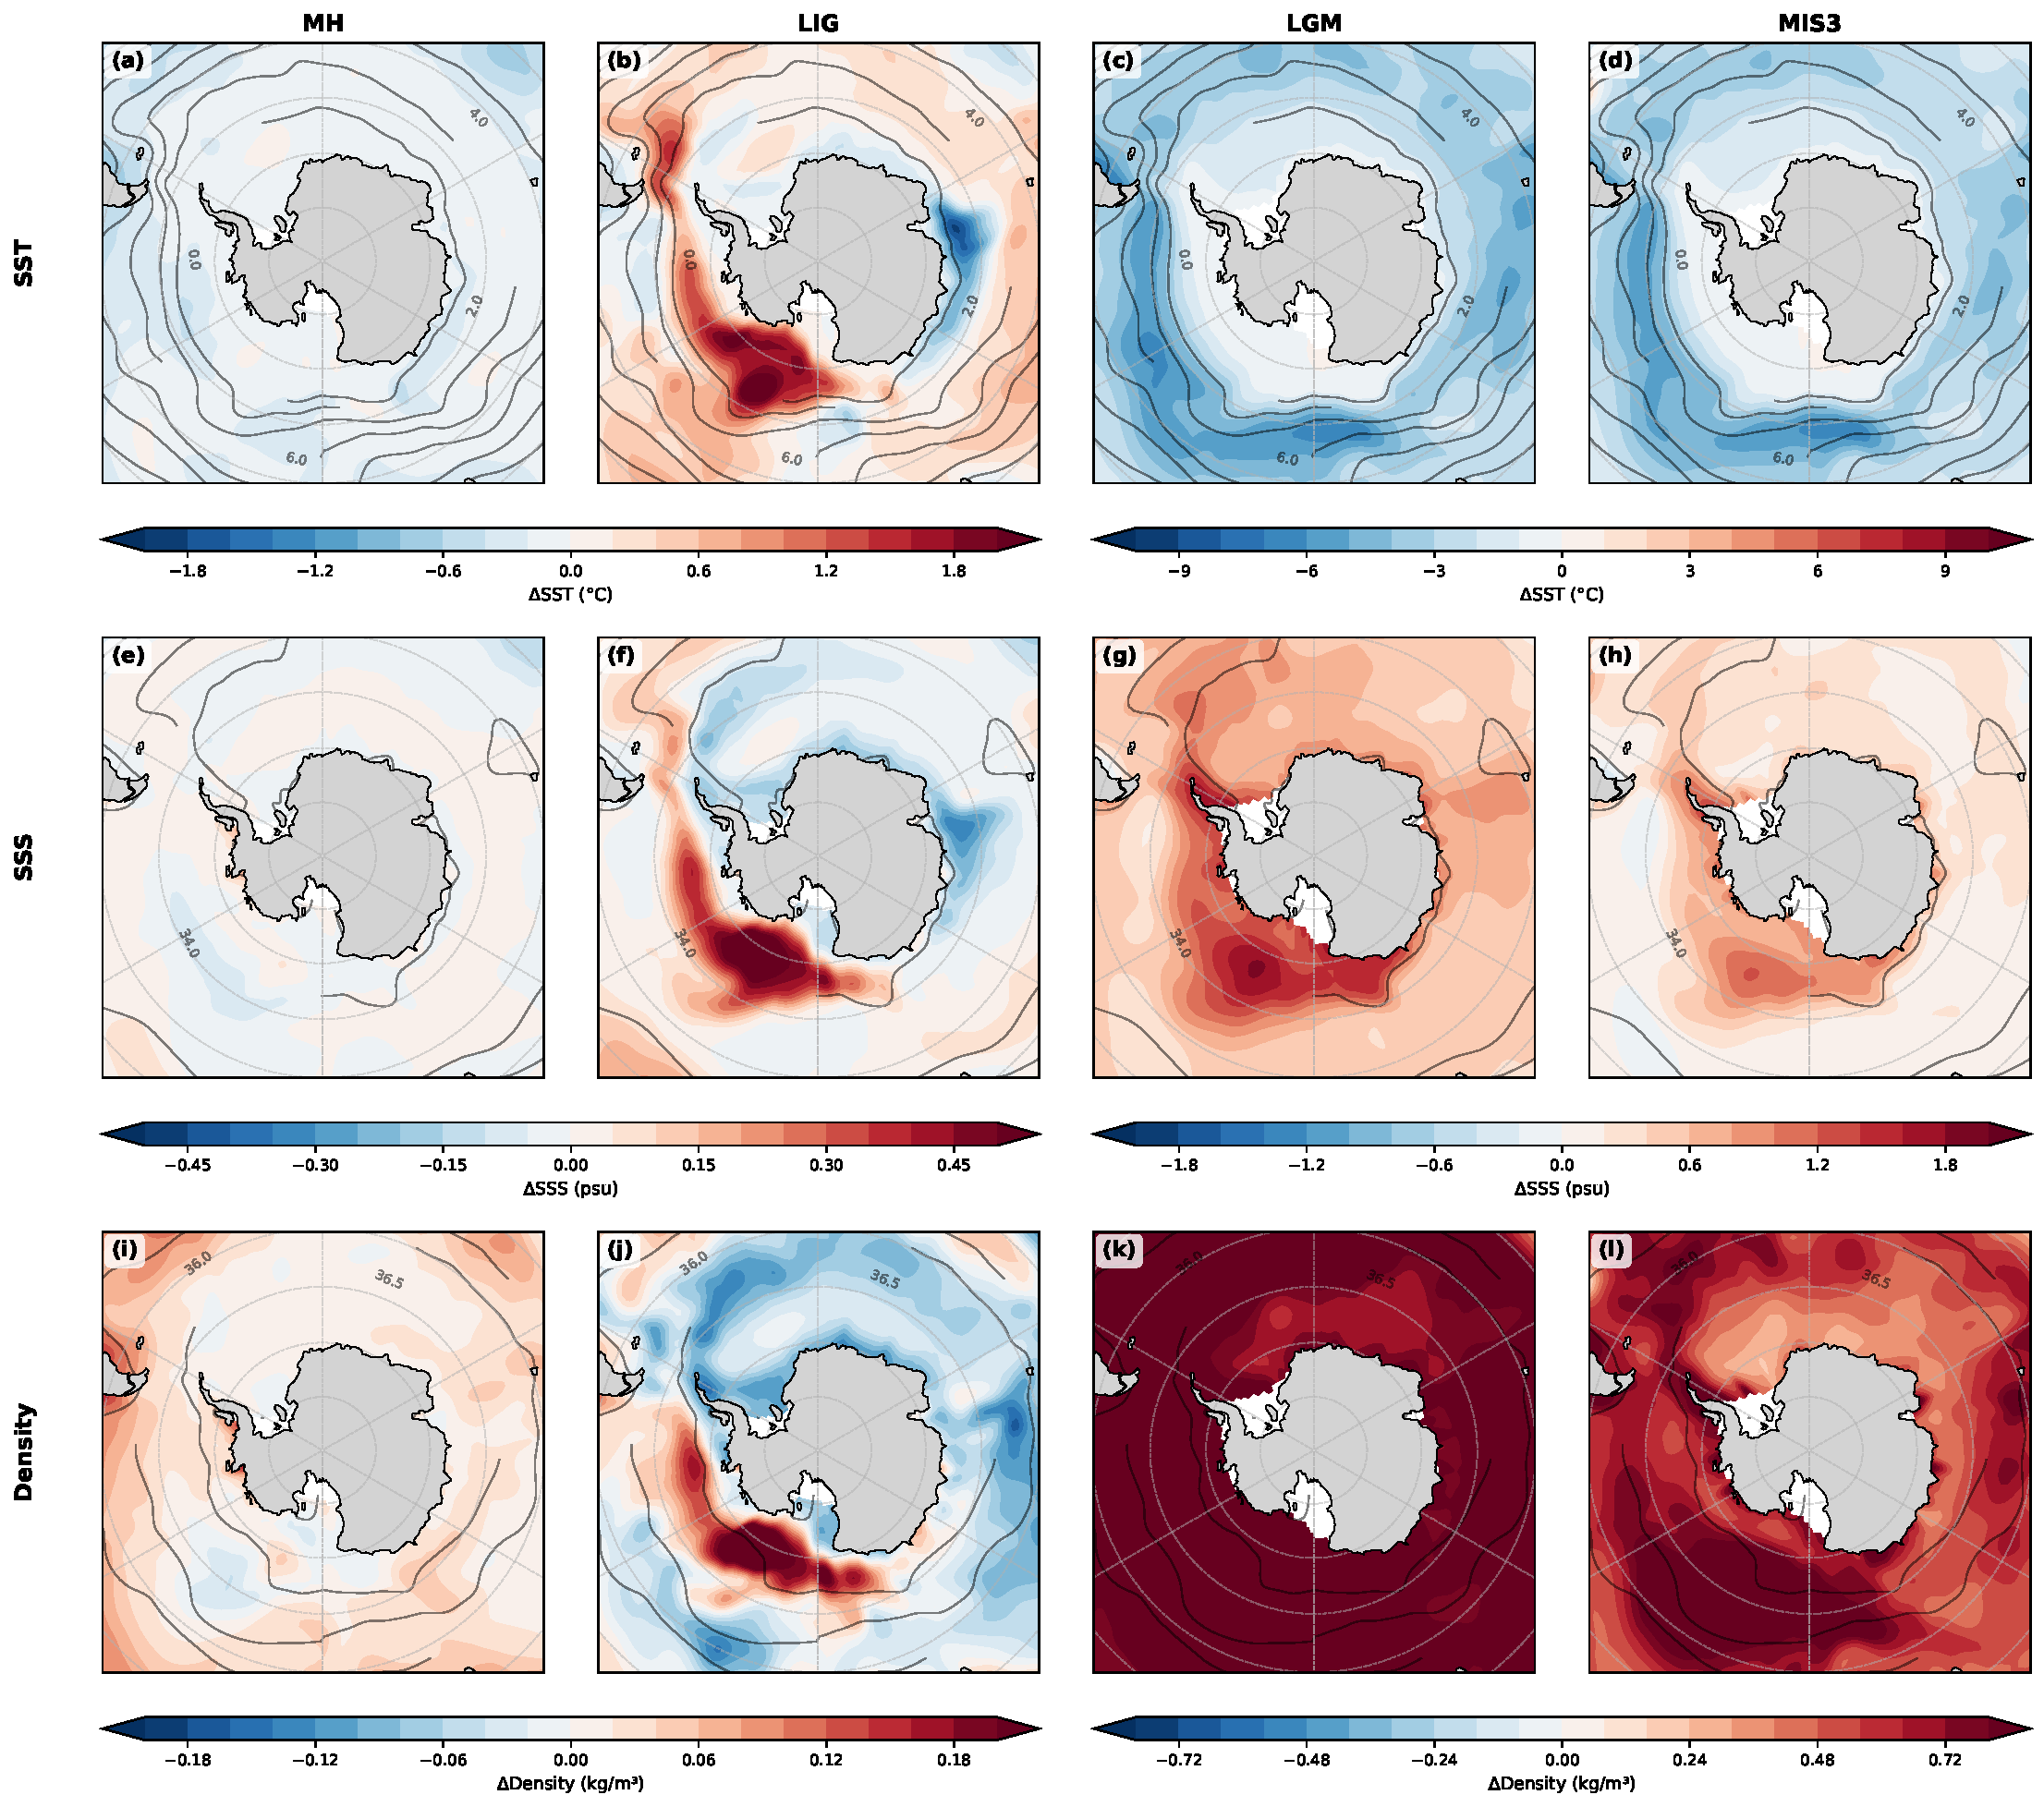
\includegraphics[width=\textwidth]{figures/fig01_climate_sst_sss_density_jja.pdf}
 \caption{Simulated anomalies in MH, LIG, LGM, and MIS3 in relative to PI for (a-d) Sea surface temperature (SST)  [$^{\circ}$C], (e-h) sea surface salinity (SSS) [psu], and (i-l) Surface density [kg/m$^3$].  \label{sst}}
\end{figure}



\begin{figure}
\centering
\includegraphics[width=\textwidth]{figures/fig02_climate_mld_seaice_jja.pdf}
\caption{Simulated JJA mean (a-e)  mixed layer depth (MLD) [m] and sea ice concentration in each experiment.  \label{mld}}
\end{figure}

\begin{figure}
\centering
\includegraphics[width=\textwidth]{figures/fig03_climate_winds_jja.pdf}
\caption{Simulated anomalies in MH, LIG, LGM, and MIS3 in relative to PI for (a-d) 10 m  zonal wind  [m/s], and (e-h) 10 m zonal wind stress [N/m$^2$]. Vectors represent PI winds and wind stress. \label{wind}}
\end{figure}


\subsection{Water mass transformation analysis}



The decomposition of water mass transformation (WMT) rates reveals a fundamental regime shift in dense water formation mechanisms between interglacial and glacial climate states (Fig. \ref{wmt_jja}).

During interglacial periods, dense water formation is predominantly thermally driven. In the austral winter (JJA), when transformation rates peak, the Southern Ocean exhibits a WMT maximum of 60--80~Sv at $\sigma_2 \approx 36.5$-$36.8$ kg m$^{-3}$ across all simulated interglacial states (Fig. \ref{wmt_jja}). This transformation is dominated by surface heat loss (red line), with limited sea ice extent restricting the haline contribution from brine rejection to a secondary role (15-30\%; green line). Other freshwater fluxes (blue lines) oppose densification through net precipitation and river runoff.

Glacial periods exhibit a distinctly different regime. The winter WMT maximum weakens substantially to 48-58 Sv while shifting to higher density classes ($\sigma_2 = 37.0$-$37.5$ kg m$^{-3}$; Fig. \ref{wmt_jja}). More fundamentally, the dominant forcing mechanism reverses, with sea ice processes contributing 15-20 Sv and constituting the majority of total WMT. This haline dominance reflects expanded sea ice coverage, which exerts dual effects on dense water formation.  Extensive ice cover insulates the ocean surface from atmospheric heat exchange, suppressing thermally driven transformation. On the other hand, enhanced sea ice production concentrates brine rejection, intensifying haline-driven densification at higher density classes ($\sigma_2 > 37$ kg m$^{-3}$). Consequently, thermal forcing operates only secondarily and at denser isopycnals, consistent with the colder glacial boundary conditions.

This interglacial thermal-dominance versus glacial haline-dominance signature is consistent across regional sectors, including the Ross Sea, Weddell Sea, and Ad\'{e}lie regions.

%This thermally dominated regime persists in the annual mean (Fig.~\ref{wmt_ann}), where net heat loss maintains a transformation rate of up to 18 Sv, balancing the seasonal buoyancy gain from summer warming.
%The glacial states mark a transition to a haline-modulated regime. While intense winter cooling remains the primary driver of instantaneous buoyancy loss (Fig.~\ref{wmt_jja}), the resulting water masses are shifted to significantly denser classes ($\sigma_2 > 37.0$~kg m${-3}$). Crucially, the role of sea ice freshwater flux shifts from a background player to a leading driver. In the annual mean (Fig.~\ref{wmt_ann}), the sea ice contribution (green line) in the LGM and MIS3 scenarios dramatically intensifies, becoming the dominant positive forcing term in the Southern Ocean and Weddell Sea sectors. This indicates that while heat loss drives the seasonal convection cycle, the expanded sea ice engine---via enhanced brine rejection---is the critical mechanism that locks these waters into the abyssal density classes.



%Regional Heterogeneity
%This mechanistic shift exhibits strong spatial heterogeneity. The Weddell Sea, serving as the classical engine of deep water formation, shows the most pronounced glacial intensification. Here, winter transformation increases to $\sim$30~Sv (at $\sigma_2 = 37.2$~kg m${-3}$), heavily reinforced by a threefold increase in sea ice-driven transformation compared to the PI state. In contrast, the Ross Sea maintains a quasi-thermal balance even under glacial conditions, suggesting that local polynya dynamics allow strong atmosphere-ocean heat fluxes to persist despite the broader expansion of the sea ice edge.




\begin{figure}
\centering
\includegraphics[width=0.9\textwidth]{figures/plot_wmt_4regions_5exps_winter_from_100years.pdf}
\caption{JJA mean water mass transformation in density space. \label{wmt_jja}}
\end{figure}



%\begin{figure}
%\centering
%\includegraphics[width=0.9\textwidth]{figures/plot_wmt_4regions_5exps_annual_from_100years.pdf}
%\caption{Annual mean water mass transformation in density space. \label{wmt_ann}}
%\end{figure}
%Annual mean WMT rates (Sv) as a function of $\sigma_2$ density for four Southern Ocean regions: Southern Ocean (sum of all), Ross Sea, Weddell Sea, and Ad\'elie Land. Each panel shows 5 experiments (PI, MH, LIG, LGM, MIS3). Lines indicate: total WMT (black), total heat flux contribution (red), sea ice freshwater contribution (teal), and other freshwater sources (blue). Interglacials show thermal dominance (70--85\% heat flux) at $\sigma_2$ = 36.6--36.8~kg/m$^3$ with modest sea ice contribution (15--30\%). Glacials shift to higher densities ($\sigma_2$ = 37.0--37.5~kg/m$^3$) with enhanced sea ice forcing (25--35\% of total), reflecting the mechanism transition from heat-dominated to haline-enhanced transformation.





\subsection{Surface density tendency from buoyancy forcing}

To identify the geographic origins and specific physical components driving the identified WMT regimes, we convert heat and freshwater fluxes into surface density tendency during austral winter (see Section 2 for more details). 

\begin{figure}
\centering
\includegraphics[width=\textwidth]{figures/surface_heat_density_tendency_from_raw_jja.pdf}
\caption{Surface density tendency caused by (a-e)  total heat flux, (f-j) radiative fluxes (SW+LW), and (k-o) turbulent component. Column 1 shows PI absolute values, and columns 2-5 show anomalies in paleo simulations relative to PI. Units: kg m$^{-3}$ s$^{-1}$. \label{density_heat}}
\end{figure}


\begin{figure}
\centering
\includegraphics[width=\textwidth]{figures/surface_freshwater_density_tendency_from_raw_jja.pdf}
\caption{Surface density tendency caused by (a-e)  total freshwater flux, (f-j) sea ice related freshwater flux, and (k-o) the total of other freshwater flux (net precipitation plus river runoff). Column 1 shows PI absolute values, and columns 2-5 show anomalies in paleo simulations relative to PI. Units: kg m$^{-3}$ s$^{-1}$. \label{density_fwf}}
\end{figure}

In PI, strong thermal densification (red shading) is concentrated along the sea ice edge and the open ocean (Fig. \ref{density_heat}a), with maximal values reaching $5 \times 10^{-6}$~kg~m$^{-3}$~s$^{-1}$ in the circumpolar band between 50-65°S. This thermal densification is overwhelmingly controlled by turbulent fluxes (sensible and latent heat), with radiative fluxes playing a minor role in the buoyancy budget (Fig. \ref{density_heat}f-j vs. Fig. \ref{density_heat}k-o). 
Interglacial anomalies (MH, LIG; Fig. \ref{density_heat}b,c,g,h,l,m) show modest changes relative to PI. MH exhibits no obvious thermal density tendency anomalies, while LIG displays localized patterns in the Ross Sea sector. This is associated with reduced sea ice coverage during LIG, allowing enhanced ocean-atmosphere heat exchange in a region that remains ice-covered during PI winter.
For glacial periods (LGM, MIS3; Fig. \ref{density_heat}d,e), despite colder atmospheric temperatures, thermal density tendency decreases throughout the Southern Ocean. Anomalies reach $-2 \times 10^{-6}$~kg~m$^{-3}$~s$^{-1}$ in the Pacific sector. This result arises from expanded glacial sea ice acting as a thermal insulating lid that prevents ocean-atmosphere heat exchange. The turbulent flux component (Fig. \ref{density_heat}n,o) shows the strongest reduction, confirming that ice cover blocks sensible and latent heat loss more effectively than radiative exchange. 

Fig. \ref{density_fwf}f exhibits a classic dipole pattern in the sea ice-driven density tendency.  Coastal divergence zones experience strong brine-driven densification while ice edge areas show weak buoyancy gain from ice melt. This pattern dominate the total haline density tendency (Fig. \ref{density_fwf}a). Other freshwater sources (net precipitation and runoff,  Fig. \ref{density_fwf}k) contribute negligibly to surface density density.
MH anomalies remain small (Fig. \ref{density_fwf}b,g,l), consistent with limited sea ice changes during MH compared to PI. During LIG, the reduced sea ice in the Ross Sea contributes to a weakening of brine rejection and therefore a weakened density tendency (Fig. \ref{density_fwf}c,h). 
Glacial periods show a pronounced northward expansion and intensification of the buoyancy loss signatures relative to PI (Fig. \ref{density_fwf}d,e,i,j). Total freshwater density tendency anomalies reach $+5 \times 10^{-9}$~kg~m$^{-3}$~s$^{-1}$ in a circumpolar band around Antarctica. The sea ice component (Fig.~5i,j) dominates this signal, with strongest anomalies in the coastal regions ($> 5 \times 10^{-9}$~kg~m$^{-3}$~s$^{-1}$).  






\subsection{Southern Annular Mode impact on water mass transformation}

\begin{figure}
\centering
\includegraphics[width=0.9\textwidth]{figures/wmt_sam_composite_4regions_5exps.pdf}
\caption{SAM composite analysis of water mass transformation (JJA).  Each panel shows total WMT anomaly (black), total heat flux contribution (red), sea ice freshwater contribution (teal), and other freshwater sources (blue).  \label{sam_wmt}}
\end{figure}
%Austral winter (JJA) water mass transformation composites showing high-SAM minus low-SAM differences (Sv) as a function of $\sigma_2$ density for four Southern Ocean regions. Panel structure: 4 rows (Southern Ocean total, Ross Sea, Weddell Sea, Ad\'elie Land) $\times$ 5 columns (PI/MH/LIG/LGM/MIS3).

                                       
The Southern Annular Mode (SAM) is the dominant mode of atmospheric variability in the Southern Hemisphere extratropics, characterized by a meridional pressure gradient between mid-latitudes and Antarctica that modulates the strength and position of the circumpolar westerlies. This atmospheric variability superimposes on mean climate states   and exerts primary control on surface buoyancy forcing, thereby governing water mass     transformation rates. Through composite analysis comparing high-SAM versus low-SAM years  (defined as JJA-mean SAM index exceeding $\pm$1.2$\sigma$ from the climatological mean)  using 100-year monthly simulations, we examine how this atmospheric forcing modulates   dense water formation across different climate states and regional sectors  (Figs.~\ref{sam_wmt}).                                                  
                                                                                          
Across all climate states, the positive phase of SAM systematically enhances WMT in the Southern Ocean (Fig.~\ref{sam_wmt}, black lines), indicating that a poleward shift and intensification of the westerlies favors dense water production. However, the magnitude and mechanism of this SAM-WMT coupling differ substantially between interglacial and glacial periods. For PI, the maximum impacts occur at $\sigma_2 = 36.7$ kg/m$^3$ with the SAM-induced WMT anomaly being 3.2 Sv,  while in MH and LIG, the maximum WMT anomaly between high and low SAM years can reach about 8 Sv, occuring at $\sigma_2 = 36.5$ kg/m$^3$, representing the strongest SAM-WMT coupling among all climate states. During glacial periods, peak anomalies are more modest (+4 Sv for LGM at $\sigma_2 = 37.5$~kg/m$^3$; +4.2 Sv for MIS at $\sigma_2 = 37.1$~kg/m$^3$) and shifted  toward higher density classes, reflecting colder and saltier background conditions.  

The partitioning between thermal and haline contributions reveals a fundamental  climate-state dependence in the SAM-WMT relationship. During interglacials, the thermal component (red lines) dominates the WMT response while the sea ice freshwater forcing plays a second role, especially in the Ross sea and Weddell sea sectors,  This thermal dominance reflects the mechanism whereby strengthened westerlies during positive SAM phases enhance turbulent heat loss at the air-sea interface, driving densification through surface cooling. In contrast, during glacial periods, sea ice freshwater flux (green lines) emerges as the primary contributor. This indicates that under extensive glacial sea ice cover, SAM-driven changes in brine rejection, rather than direct heat loss, become the dominant process for modulating dense water formation.   

Regional decomposition reveals that the Weddell Sea and Ad\'elie sectors contribute consistently to the circumpolar SAM-WMT signal across interglacial climate states, while the Ross Sea exhibits more variable and sometimes opposing responses. Moreover, the glacial WMT response to SAM is overall dominated by the Weddell Sea region, whereas the Ross Sea and Ad\'elie sectors play a minor role. These regional  heterogeneities reflect differences in local sea ice dynamics, and circulation patterns that modulate how atmospheric forcing translates to surface        
  buoyancy changes.                                                                           
                          
                                                                                    
To understand the mechanisms underlying these SAM-WMT relationships, we now turn to examine the spatial patterns of surface heat flux and freshwater flux anomalies between high and low SAM composite years.

Heat flux composites reveals  distinct responses between interglacial and glacial periods (Fig.\ref{sam_heat}). During interglacials, positive SAM phases systematically enhance ocean heat loss by more than 15~W/m$^2$ across the high-latitude ice-free  Southern Ocean where open water permits direct atmosphere-ocean coupling  (Fig.~\ref{sam_heat}), particularly in the Weddell Sea, the Bellingshausen Sea, and the Indian Ocean sector. Decomposition into components shows that turbulent fluxes (sensible and latent heat fluxes) account for most of this anomaly, while radiative contributions (longwave and shortwave fluxes) remain negligible.  In contrast, glacial periods (LGM and MIS3) show only weak SAM-driven changes across at high-latitudes, as extensive sea ice coverage limits direct atmosphere-ocean exchange.


Freshwater flux composites indicate that SAM influences dense water formation primarily through sea ice processes rather than net precipitation or river runoff (Fig.~\ref{sam_fwf}). Total freshwater flux anomalies exhibit general dipole patterns with positive SAM driving freshwater loss (ocean salinification) in coastal regions accompanied by freshwater gain offshore. This pattern is controlled by sea ice processes. Under high-SAM conditions, strengthened winds enhance offshore sea ice transport and ice formation in coastal polynyas, leading to intensified brine rejection.

Together, these results demonstrate that SAM systematically modulates WMT rates across all the 5 simulated climate states through two distinct contributors: thermal forcing, which dominates during interglacials via turbulent heat fluxes, and haline forcing, which dominates during glacials via sea ice processes.



%Climate state dependency is pronounced. Interglacial periods (PI/MH/LIG) exhibit spatially coherent positive heat flux anomalies throughout the ice-free Southern Ocean, with maximum values in the Atlantic and Indian sectors where open water permits direct atmosphere-ocean coupling. In contrast, glacial periods (LGM/MIS3) show reduced SAM-driven heat flux variability due to expanded sea ice insulation that dampens atmosphere-ocean exchange. The heat flux anomaly magnitude decreases by approximately 40\% during glacials compared to interglacials, demonstrating that sea ice extent fundamentally modulates SAM's capacity to influence surface buoyancy forcing.

%Regional patterns reflect local oceanographic conditions. The Ross Sea exhibits the strongest SAM sensitivity during interglacials, with heat flux anomalies exceeding 20~W/m$^2$ during high-SAM phases---consistent with this region's exposure to westerly wind variability and reduced sea ice buffering during warm periods. The Weddell Sea shows more muted response due to persistent open-water areas that maintain atmosphere-ocean coupling even during low-SAM conditions. This regional heterogeneity implies that SAM-driven WMT changes concentrate in specific sectors rather than occurring uniformly around Antarctica.

\begin{figure}
\centering
\includegraphics[width=\textwidth]{figures/sam_heatflux_composite_t63_3rows_5cols.pdf}
\caption{Austral winter (JJA) mean surface heat flux anomalies for high-SAM minus low-SAM composites (1$\sigma$ threshold) across five paleoclimate states.  Row 1: Total heat flux (all components combined). Row 2: Radiative component (longwave + shortwave). Row 3: Turbulent component (sensible + latent heat). Units: W/m$^2$ from ocean perspective (positive indicates reduced ocean heat loss during high-SAM).\label{sam_heat}}
\end{figure}
%Panel structure: 3 rows × 5 columns (PI/MH/LIG/LGM/MIS3).  High-SAM conditions systematically enhance ocean heat loss (negative anomalies, blue colors) exceeding 15~W/m$^2$ in the circumpolar 50--65°S band. Turbulent fluxes contribute 60--70\% of total anomaly. The Ross Sea exhibits strongest SAM sensitivity during interglacials (>20~W/m$^2$), consistent with reduced sea ice buffering.

\begin{figure}
\centering
\includegraphics[width=\textwidth]{figures/sam_fwflux_composite_3rows_5cols.pdf}
\caption{Austral winter (JJA) mean freshwater flux anomalies for high-SAM minus low-SAM composites (1$\sigma$ threshold) across five paleoclimate states.  Row 1: Total freshwater flux. Row 2: Sea ice component (brine rejection and melt). Row 3: Other sources (net precipitation + runoff). Units: mm/day (positive indicates net freshwater gain to ocean, negative indicates salinification). \label{sam_fwf}}
\end{figure}

%High-SAM drives complex dipole patterns with coastal freshwater loss (salinification from enhanced brine rejection) and offshore gain (from ice melt). The sea ice component (row 2) dominates other sources (row 3) by factors of 3--5, confirming that SAM influences WMT primarily through haline forcing via sea ice redistribution. Glacial periods exhibit amplified responses ($>$1.0~mm/day) due to expanded baseline sea ice coverage providing larger reservoir for SAM-driven redistribution.



%The sea ice freshwater component dominates other sources (net precipitation and river runoff) in all climate states, confirming that SAM-driven WMT variability operates primarily through haline forcing via sea ice redistribution. Glacial periods exhibit amplified sea ice responses: LGM and MIS3 show freshwater flux anomalies exceeding 1.0~mm/day in coastal regions during high-SAM phases, compared to 0.5--0.7~mm/day in interglacials. This glacial amplification reflects expanded baseline sea ice coverage providing larger reservoir for SAM-driven redistribution.

%Seasonal dependence is critical. Winter composites (JJA) show strongest signals when sea ice formation peaks, whereas summer patterns (not shown) exhibit reversed but weaker anomalies associated with melt season dynamics. The asymmetry between winter intensification and summer weakening creates net annual haline forcing that persists beyond individual SAM events, potentially influencing dense water properties on multi-year timescales.



\subsection{Ventilation age simulations}





\begin{figure}
\centering
\includegraphics[width=\textwidth]{figures/age_horizontal_3900m.pdf}
\caption{Horizontal distribution of ideal age (years) at 3900 m depth for five experiments. \label{age_abs}}
\end{figure}
 


\begin{figure}[h]
\centering
\includegraphics[width=\textwidth]{figures/age_horizontal_3900m_anomaly.pdf}
\caption{Simulated anomalies in ideal age (years) at 3900 m depth (paleo minus PI). \label{age_anm}}
\end{figure}


%\textbf{Figure 12: Vertical profiles of ideal age by ocean basin.}
%\begin{figure}[h]
%\centering
%\includegraphics[width=0.8\textwidth]{figures/age_vertical.pdf}
%\end{figure}
%Basin-averaged vertical age profiles (years vs depth) for Atlantic, Indian, and Pacific oceans across five experiments. Interglacials show modest depth-increasing ages: Atlantic/Indian 500--750~yr at 4000~m, Pacific 800--1200~yr. Glacials exhibit systematically older ages with strong depth dependence: Atlantic reaches 1500--2000~yr, Pacific exceeds 2500~yr below 3000~m (tripling relative to PI). Indian Ocean shows intermediate behavior. These profiles quantify basin-specific ventilation changes and demonstrate that Pacific deep waters experience most dramatic aging under glacial conditions due to remoteness from Southern Ocean formation regions.

%\textbf{Figure 13: Vertical profiles of ideal age anomalies by ocean basin.}
%\begin{figure}[h]
%\centering
%\includegraphics[width=0.8\textwidth]{figures/age_vertical_anm.pdf}
%\end{figure}
%Basin-averaged age anomaly profiles (years vs depth, relative to PI). MH exhibits minimal anomalies ($<\pm$100~yr). LIG shows slight rejuvenation in Atlantic ($-$75 to $-$150~yr throughout water column) from enhanced dense water formation, while Pacific shows modest increases (+100~yr deep). Glacials display depth-increasing anomalies: LGM/MIS3 reach +1500~yr in deep Pacific, +800~yr in Atlantic, +500~yr in Indian. The systematic depth-dependence reflects reduced ventilation at depth where sluggish abyssal circulation magnifies the impact of reduced formation rates. These anomaly profiles isolate pure climate-driven ventilation changes independent of baseline circulation structure.

Having examined surface water mass transformation, we next assess deep ocean ventilation through ideal age distributions at 3900 m depth Fig.\ref{age_abs}-\ref{age_anm}.


Ideal age distributions at 3900~m depth reveal fundamental restructuring of abyssal ventilation across different climate states (Fig.\ref{age_abs}-\ref{age_anm}). Interglacial periods are characterized by relatively young deep waters. PI, MH, and LIG all exhibit ages below 500 yr in the Atlantic and Indian sectors, with the oldest waters (> 500yr) confined to the Pacific. Among interglacials, MH exhibits minimal age changes relative to PI, suggesting similar dense water formation rates. LIG anomalies reveal younger-than-PI ages (up to $-$150~yr) in the Belingshausen Sea sector, attributed to reduced sea ice coverage and enhanced thermal forcing. In contrast, the Atlantic and Indian Ocean sectors show modest age increases during LIG (less than 70 yr). Glacial periods exhibit different patterns. LGM and MIS3 ages exceed 750 yr throughout the Atlantic and Indian basins, with Pacific ages reaching 1500 ~yr. This represents a significant global increase in deep ocean isolation in glacial times, consistent with radiocarbon proxy reconstructions \citep{Skinner2017}.


%Vertical age profiles quantify basin-specific ventilation changes (Fig.~12). In the Atlantic, glacial ages increase systematically with depth, reaching 1500--2000~yr at 4000~m compared to 500--750~yr in interglacials. The Indian Ocean shows intermediate behavior. Most striking is the Pacific, where glacial ages exceed 2500~yr below 3000~m---a tripling relative to PI. Age anomaly profiles (Fig.~13) isolate climate-driven changes: LIG shows slight rejuvenation throughout the water column in the Atlantic ($-$75 to $-$150~yr), while LGM/MIS3 exhibit depth-increasing anomalies reaching $+$1500~yr in the deep Pacific. These patterns reflect enhanced stratification and altered circulation under glacial boundary conditions.


% ============================================================================
% Discussion
% ============================================================================
\section{Discussion}



\subsection{Southern Annular Mode influence on AABW formation}

\subsubsection{Implications for AABW variability and predictability}

These SAM composite results provide mechanistic basis for understanding observed decadal AABW variability. Recent observations document 30\% reduction in Weddell Sea AABW formation since 1992 linked to wind-driven sea ice decline \citep{Zhou2023}, while Ross Sea exhibited recovery during 2015--2019 from positive SAM combined with El Niño forcing \citep{Silvano2020}. Our analysis demonstrates that such SAM-driven changes operate consistently across all climate states, with high-SAM systematically enhancing formation through combined heat loss and sea ice intensification.

The persistent SAM-AABW relationship across glacial-interglacial cycles implies potential for paleoclimate proxy development. If SAM variability influences formation rates by 15--20\% on multi-year timescales, and formation changes propagate to deep ocean tracer signatures, then high-resolution sediment core records from AABW formation regions might preserve SAM-frequency variability. Existing radiocarbon and benthic isotope records rarely achieve sub-centennial resolution, but emerging techniques (e.g., paleointensity-assisted chronologies, annual-layer counting in high-accumulation sites) could enable SAM reconstruction extending beyond instrumental period.

Furthermore, climate models' ability to capture SAM-AABW coupling provides validation metric for model physics. Models that correctly simulate SAM-driven surface flux anomalies and their translation to WMT changes demonstrate realistic representation of atmosphere-ocean-sea ice interactions critical for projecting future AABW response to Southern Hemisphere climate change. Our results establish quantitative benchmarks (15--20\% WMT modulation, 70--80\% thermal contribution in interglacials shifting to 60--65\% in glacials) against which model performance can be assessed.



<<<<<<< HEAD
Our systematic water mass transformation analysis across five paleoclimate states reveals fundamental mechanisms governing AABW formation response to climate forcing and provides insights into deep ocean ventilation changes that controlled past carbon storage. Here we synthesize our findings within the broader context of observational constraints, proxy reconstructions, and theoretical understanding, while carefully addressing model limitations and their implications for interpreting results.

\subsection{Mechanism-based insights despite model representation limitations}

Climate models face well-documented challenges in representing AABW formation processes. As discussed in Section 1.6, most CMIP6 models---including AWI-ESM---form AABW predominantly through open-ocean deep convection rather than realistic shelf overflow processes \citep{Heuze2021, deLavergne2014}. This limitation stems from insufficient horizontal resolution to resolve shelf processes, which require approximately 2--4~km resolution \citep{Schmidt2025}. The absence of explicit dense water cascades and polynya dynamics introduces systematic biases in formation location, seasonality, and potentially sensitivity to forcing.

However, recent advances in paleoclimate science demonstrate that \textbf{models with known biases can still provide valuable mechanistic insights when their limitations are properly acknowledged and analysis focuses on process understanding rather than precise quantification} \citep{Zhu2021NCC}. The paleoclimate record provides ``out-of-sample'' tests for climate models under conditions of substantial CO$_2$ change, allowing evaluation of fundamental physics and feedbacks that operate on centennial-plus timescales inaccessible to the instrumental record \citep{Tierney2020Paleo}. Critically, \citet{Zhu2021NCC} emphasize that paleoclimate data represent complementary constraints to modern observations, with the combination of both reducing potential model biases in future projections. Similarly, recent analysis shows that CMIP6/PMIP4 ensemble means successfully simulate global mean surface temperatures across multiple paleoclimate periods, with paleoclimate data identifying and correcting specific parameterization issues---for example, excessive climate sensitivity in CESM2 was diagnosed and remedied through paleoclimate evaluation revealing cloud parameterization problems.

\textbf{Our analysis strategy explicitly accounts for model limitations through comparative mechanism diagnosis rather than absolute formation rate quantification.} We focus on three aspects where mechanistic insights remain robust despite open-ocean convection biases:

\textbf{(1) Relative changes in forcing mechanisms across climate states.} While absolute WMT magnitudes may differ from observations, the \textit{shift} from heat-flux dominance (85--90\% contribution) during interglacials to enhanced haline forcing (25--30\% sea ice contribution) during glacials reflects fundamental thermodynamic responses to boundary condition changes. This mechanism transition---thermal cooling in ice-free regions versus brine rejection in ice-covered polynya-like areas---operates regardless of whether formation occurs via shelf overflow or open-ocean convection. The physics of surface buoyancy flux partitioning under different sea ice regimes is robust across formation pathways.

\textbf{(2) Sea ice's dual role in modulating surface forcing.} Our decomposition reveals that glacial sea ice expansion simultaneously (a) insulates the bulk ocean surface from atmospheric heat loss and (b) concentrates brine rejection in localized formation regions. This dual thermal-insulation and haline-intensification mechanism represents fundamental sea ice physics captured even in models with imperfect formation geography. Recent observational studies confirm this dual role: expanded Weddell Sea ice reduces area-integrated ocean heat loss while coastal polynyas maintain intense brine rejection \citep{Bailey2023}, and interannual sea ice variability drives 30\% changes in AABW formation through combined thermal and haline pathways \citep{Zhou2023}.

\textbf{(3) Ventilation age response to circulation changes.} Ideal age distributions integrate the cumulative effect of formation rate changes, transport pathways, and mixing---the age increase of $\sim$1500~yr during glacials primarily reflects reduced formation and enhanced stratification rather than specific formation mechanism details. Model-data radiocarbon comparison (Section 4.2) demonstrates consistency with proxy constraints despite formation location biases, suggesting that basin-scale ventilation response is less sensitive to sub-grid-scale formation processes than might be expected.

This approach aligns with emerging best practices in paleoclimate modeling. Regional climate model studies acknowledge that ``model biases, either from regional climate models themselves or inherited from the driving global model, usually remain'' but emphasize that relative changes and process understanding retain value \citep{Fallah2016}. Similarly, recent assessments emphasize that paleoclimates provide essential tests for latest-generation climate models precisely because models developed primarily from modern observations require out-of-sample validation to identify hidden biases \citep{Zhu2021NCC}. Our focus on \textit{mechanisms}---how thermal versus haline forcing shifts with sea ice coverage, how stratification responds to source water density changes---rather than precise formation rates aligns with this paradigm of extracting robust insights from imperfect models.

\subsection{Comparison with geological proxy reconstructions}

Our simulated ventilation age changes across paleoclimate states can be directly compared with multiple independent geochemical proxy constraints, providing validation of model-diagnosed circulation changes despite formation mechanism limitations discussed above.

\subsubsection{Radiocarbon-based ventilation ages}

Benthic-planktonic $^{14}$C age offsets from sediment cores reveal that glacial deep ocean radiocarbon ages increased globally, with the strongest signals in the Pacific and Southern Ocean \citep{Skinner2010, Skinner2017}. Our simulated LGM ideal age increase of $\sim$1500~yr at 3900~m depth (Fig.~10--11) compares favorably with radiocarbon-derived estimates: \citet{Skinner2017} report that glacial deep ocean $^{14}$C-ventilation ages increased by approximately 689$\pm$53~$^{14}$C-yr compared to the Holocene, with southern-sourced abyssal waters particularly isolated. However, direct comparison requires careful interpretation because benthic-planktonic $^{14}$C ages comprise both true circulation age and ``preformed $^{14}$C-age'' arising from incomplete atmosphere-ocean equilibration at formation regions \citep{Koeve2015}. The sea ice-covered glacial Southern Ocean likely experienced substantial surface reservoir age increases (up to several hundred years), inflating apparent ventilation ages \citep{Skinner2019}.

Recent high-resolution studies provide more nuanced constraints. \citet{Li2024CP} used transient deglacial simulations with both radiocarbon and ideal age tracers to demonstrate that \textit{true} (ideal) ventilation age peaked around 14--12~ka during weakened AABW transport, reaching 1900--2200~years---substantially older than LGM values. This apparent paradox---younger ideal age at LGM despite older radiocarbon age---reflects that enhanced glacial brine rejection drove stronger AABW transport that partially compensated for expanded sea ice insulation effects. Our results support this interpretation: glacial WMT shifts to higher density classes ($\sigma_2$ = 37.0--37.5~kg/m$^3$ versus 36.6--36.8~kg/m$^3$), producing denser source waters that sink more readily despite reduced area-integrated heat loss.

The most recent work further refines understanding. A 2025 \textit{Nature Communications} study demonstrates that reduced AABW overturning during early deglaciation produced the ``radiocarbon ventilation seesaw'' between Atlantic and Pacific basins, with AABW weakening causing Atlantic ventilation age increases while Pacific ages decreased due to compensating NADW changes. Our regional age distributions (Fig.~11--13) capture similar basin-specific responses: LGM shows maximum age increases in the deep Pacific (+1500~yr) where remoteness from formation regions amplifies circulation slowdown effects, while the Atlantic exhibits more modest increases (+800~yr) due to proximity to both NADW and AABW sources.

\subsubsection{Neodymium isotopes and water mass geometry}

Neodymium isotopes ($\epsilon_{Nd}$) provide complementary constraints on deep water mass geometry that are less affected by reservoir age complications. Modern AABW displays radiogenic $\epsilon_{Nd}$ signatures ($\sim$-8 to -7) distinct from unradiogenic NADW ($\sim$-13), allowing reconstruction of relative contributions \citep{Lambelet2016}. Compilation of benthic foraminiferal $\epsilon_{Nd}$ across glacial-interglacial cycles reveals oscillating NADW versus AABW influence, with AABW maximized during stadials \citep{Piotrowski2008, Huang2020}.

While our model does not include explicit neodymium cycling, our simulated circulation changes imply corresponding $\epsilon_{Nd}$ variations that can be qualitatively assessed. During LGM, our enhanced AABW formation intensity in the dense water classes combined with increased ventilation ages suggests expanded AABW volume filling the abyssal Atlantic---consistent with $\epsilon_{Nd}$ evidence for NADW shoaling to $\sim$2000~m and AABW expansion \citep{Curry2005, Hines2021}. The regional heterogeneity we diagnose (strong Weddell enhancement, modest Ross response; Section 3.3) aligns with sediment core evidence showing Atlantic sector dominance of glacial AABW export \citep{Piotrowski2005}.

Recent modeling studies incorporating neodymium cycling confirm that $\epsilon_{Nd}$ variations primarily track NADW versus AABW formation rate changes rather than boundary exchange artifacts \citep{Gu2019, Poppelmeier2022}, validating use of $\epsilon_{Nd}$ for circulation reconstruction. Our mechanism diagnosis---that glacial sea ice drives the thermal-to-haline shift producing denser AABW---provides process-level explanation for proxy-observed circulation restructuring. Specifically, the denser glacial source waters (0.3--0.5~kg/m$^3$ increase) we diagnose would propagate farther and resist mixing more effectively, potentially explaining $\epsilon_{Nd}$ evidence for expanded glacial AABW footprint \citep{Hines2021}.

\subsubsection{Benthic carbon isotopes and respired carbon storage}

Benthic foraminiferal $\delta^{13}$C distributions reveal that the glacial deep ocean stored substantially more respired carbon, with low $\delta^{13}$C values indicating nutrient- and CO$_2$-rich waters \citep{Curry1988, OppoFairbanks1987}. Atlantic $\delta^{13}$C compilations show dramatic restructuring at LGM, with a strong vertical gradient consistent with shoaled NADW and expanded nutrient-rich AABW \citep{Curry2005}. Our ventilation age results directly support this carbon storage mechanism: 1500-year age increases imply prolonged isolation from atmospheric CO$_2$ exchange, allowing accumulation of respired carbon from remineralization of sinking organic matter. Combined with enhanced stratification from denser source waters, this creates conditions for efficient deep ocean carbon sequestration potentially explaining 50--80~ppm of glacial-interglacial CO$_2$ variations \citep{Skinner2017, Ferrari2014}.

Recent radiocarbon-$\delta^{13}$C synthesis demonstrates that the glacial Atlantic stored enhanced respired carbon specifically in the depth range 2000--4000~m where AABW replaced NADW \citep{Skinner2016}. Our simulated depth-dependent age increases (Fig.~12--13) match this pattern: maximum aging occurs at abyssal depths where AABW dominates, while shallower depths show more modest changes reflecting NADW-AABW competition. The mechanism we diagnose---sea ice-driven shift to haline-enhanced, denser AABW formation---provides the physical driver for this biogeochemical restructuring.

\subsubsection{Regional proxy evidence and model-data synthesis}

Beyond basin-scale patterns, regional proxy compilations enable more detailed model-data comparison. Our simulated LIG Ross Sea age anomaly (up to -150~yr younger than PI; Fig.~11) reflects reduced sea ice coverage and enhanced thermal forcing in this sector. While high-resolution proxy records from the Ross Sea spanning LIG remain limited, existing evidence suggests enhanced polynya activity and potential AABW intensification during warm periods \citep{McKay2012}, qualitatively consistent with our mechanism diagnosis. Conversely, Weddell Sea sediment cores document persistent AABW export throughout interglacials with modest variability \citep{Hayes2014}, matching our simulated modest age changes in this region during MH/LIG.

Synthesizing across multiple proxy types---radiocarbon ages, $\epsilon_{Nd}$, $\delta^{13}$C, and regional records---our model-diagnosed mechanisms achieve first-order consistency with geological constraints. The simulated 1500-year ventilation age increase, thermal-to-haline forcing transition, and regional heterogeneity align with independent proxy evidence despite model limitations in formation processes. This consistency supports our central conclusion that sea ice governs AABW's climate response through its dual thermal-insulation and haline-intensification roles.

\subsection{Theoretical understanding and mechanistic synthesis}

Our results illuminate theoretical predictions for how AABW responds to climate forcing, connecting to fundamental frameworks for Southern Ocean dynamics.

\subsubsection{Water mass transformation theory and observations}

The WMT framework \citep{Walin1982, Groeskamp2019} provides thermodynamic basis for relating surface buoyancy fluxes to dense water formation rates. Our decomposition into individual heat and salt components (Section 3.2--3.3) extends recent observational WMT applications \citep{Pellichero2018, Bailey2023} into paleoclimate domain. Critically, \citet{Pellichero2018} used Argo floats and instrumented seals to show that seasonal sea ice growth and melt dominates water mass transformation in the ice-covered sector, with freshwater fluxes rather than heat fluxes driving meridional overturning feeding AABW formation---observing approximately 5$\pm$5~Sv transformation into denser AABW classes. Our interglacial results show comparable WMT magnitudes (5--8~Sv winter transformation at $\sigma_2$ = 36.6--36.8~kg/m$^3$; Fig.~9) but with heat flux dominance (70--80\% thermal contribution) rather than freshwater dominance.

This apparent discrepancy reflects different spatial domains and temporal averaging. \citet{Pellichero2018} integrated over the entire ice-covered Southern Ocean including the strong freshwater-driven upper cell transformation, whereas our focus on dense water classes ($\sigma_2$ $>$ 36.5~kg/m$^3$) isolates the AABW precursor formation specifically. Regional analysis by \citet{Bailey2023} for the Weddell Sea demonstrates that sea ice brine rejection dominates surface salt flux throughout most seasons, consistent with our glacial results showing 25--30\% sea ice contribution. The climate-dependent partitioning we diagnose---interglacial thermal dominance versus glacial haline enhancement---reflects that expanded sea ice fundamentally restructures the relative importance of formation pathways.

\subsubsection{Sea ice-ocean-atmosphere coupling and climate feedbacks}

Sea ice's dual role illuminated by our analysis connects to theoretical understanding of polar ocean-atmosphere coupling. The thermal insulation effect we diagnose (glacial ocean experiencing reduced heat loss despite colder air; Fig.~4) has been recognized in sea ice physics for decades but rarely quantified in paleoclimate WMT context. \citet{Abernathey2016} described sea ice as a ``freshwater pump'' that removes freshwater from high latitudes through equatorward transport and melting, concentrating salt in formation regions. Our surface flux decomposition (Fig.~6--7) demonstrates this pump operating with enhanced intensity during glacials: coastal brine rejection intensifies while offshore melting decreases, creating spatial partitioning that localizes dense water formation.

This sea ice-mediated forcing restructuring creates a climate feedback: expanded glacial sea ice $\rightarrow$ reduced area-integrated heat loss but intensified localized brine rejection $\rightarrow$ formation shifts to higher density classes $\rightarrow$ denser AABW spreads farther and resists mixing $\rightarrow$ enhanced stratification isolates deep ocean $\rightarrow$ reduced CO$_2$ outgassing $\rightarrow$ contributes to maintaining expanded sea ice. This positive feedback loop potentially explains the persistence of glacial deep ocean isolation documented in proxy records \citep{Ferrari2014, Jansen2017}. Breaking this feedback during deglaciations likely requires external forcing (orbital changes, ice sheet collapse, freshwater discharge) rather than internal variability \citep{Sigman2021}.

\subsubsection{SAM variability and decadal-to-centennial modulation}

Our SAM composite analysis (Section 3.5) demonstrates that atmospheric variability modulates AABW formation by 15--20\% on multi-year timescales across all climate states. This provides mechanistic explanation for observed decadal changes: 30\% Weddell Sea AABW reduction since 1992 linked to wind-driven sea ice decline \citep{Zhou2023}, and 2015--2019 Ross Sea recovery from positive SAM combined with El Niño forcing \citep{Silvano2020}. Critically, our finding that SAM-AABW coupling persists across glacial-interglacial cycles with similar relative sensitivity (despite dramatically different background conditions) suggests fundamental atmosphere-ocean-sea ice physics operating independently of climate state.

This has implications for interpreting proxy records. If SAM variability consistently modulates formation by 15--20\%, high-resolution sediment cores from AABW formation regions should preserve sub-centennial variability reflecting past SAM fluctuations. Existing radiocarbon records rarely achieve this resolution due to bioturbation and dating uncertainties, but emerging techniques (paleointensity-assisted chronologies, annual-layer counting in high-accumulation sites) could enable SAM reconstruction extending beyond instrumental records. Such reconstructions would test whether SAM frequency and amplitude changed across climate states---a critical unknown for understanding Southern Hemisphere climate dynamics.

\subsection{Implications for future climate projections}

While our study focuses on paleoclimate states, the mechanistic insights have direct relevance for projecting 21st-century deep ocean changes.

\subsubsection{Antarctic meltwater forcing and formation pathway shifts}

Projected Antarctic ice sheet mass loss could discharge substantial freshwater into AABW formation regions, with modeling studies suggesting more than 40\% abyssal overturning slowdown by 2050 under high-emission scenarios \citep{Li2023Nature}. Our analysis indicates this freshwater forcing would not simply weaken formation but rather \textit{shift formation mechanisms}---potentially toward even more haline-dominated pathways if sea ice responses amplify brine rejection in remaining formation regions. However, the nonlinearity is critical: beyond a threshold freshwater flux, stratification could prevent convection entirely, as observed in the Amundsen Sea where glacial meltwater halts deep water formation despite active polynyas \citep{Silvano2018}.

Our paleoclimate results provide constraints on this threshold. During LIG---our warmest simulation with reduced sea ice---Ross Sea formation continued with enhanced thermal forcing rather than shutting down, suggesting that moderate warming intensifies rather than eliminates formation. However, transient freshwater pulses during deglaciation (not captured in our equilibrium simulations) caused millennial-scale AABW weakening events \citep{Hayes2014, Glasscock2020}, indicating that \textit{rate} of change matters beyond equilibrium state. Future projections require transient simulations with realistic ice sheet-ocean coupling to capture threshold behavior.

\subsubsection{Climate model evaluation metrics from paleoclimate constraints}

Our mechanistic benchmarks provide quantitative targets for evaluating climate models used in future projections. Models that correctly simulate: (1) thermal-to-haline forcing transition with sea ice expansion (interglacial 85--90\% thermal shifting to glacial 70--75\% thermal, 25--30\% haline); (2) sea ice's dual thermal-insulation and haline-intensification roles; (3) SAM-driven 15--20\% WMT modulation across climate states; and (4) ventilation age increases of $\sim$1500~yr during glacial expansion---demonstrate realistic atmosphere-ocean-sea ice coupling essential for credible future projections.

Recent paleoclimate-based model evaluation \citep{Zhu2021NCC} shows that models passing paleoclimate tests exhibit reduced uncertainty in future projections, with paleoclimate constraints cutting projected warming ranges by approximately 30\%. Applying similar methodology to AABW specifically---using our WMT mechanism metrics as evaluation criteria---could identify which CMIP7 models most reliably project future deep ocean circulation changes. This is critical because inter-model spread in projected AABW response currently spans factors of 2--3 \citep{Heuze2021}, limiting confidence in climate impact assessments.





\subsection{Implications for understanding deep water formation}

While our analysis characterizes surface forcing rather than AABW formation directly, the results have implications for understanding how deep water formation mechanisms may respond to climate change.

\subsubsection{Sea ice as a key modulator}

The dual role of sea ice---thermal insulation combined with brine concentration---suggests that sea ice extent and distribution exert strong control on dense water formation regardless of specific formation pathways. Our finding that glacial sea ice expansion reduces area-integrated heat loss while intensifying localized haline forcing is consistent with the \citet{Abernathey2016} conceptualization of sea ice as a ``freshwater pump.'' This mechanism likely operates in both modeled open-ocean convection and real-world shelf processes, suggesting that the thermal-to-haline forcing shift we diagnose may be qualitatively robust.

\subsubsection{SAM influence on Southern Ocean processes}

The 15--20\% SAM modulation of WMT we diagnose provides context for understanding observed decadal variability. Recent observations document 30\% reduction in Weddell Sea deep water formation since 1992 linked to wind-driven sea ice decline \citep{Zhou2023}, and 2015--2019 Ross Sea recovery from positive SAM \citep{Silvano2020}. Our finding that SAM-WMT coupling persists across climate states with similar relative sensitivity suggests this represents fundamental atmosphere-ocean-sea ice physics. This provides both a model evaluation metric and context for interpreting observed variability.

\subsubsection{Paleoclimate context for future projections}

Projected Antarctic ice sheet mass loss could substantially modify dense water formation through freshwater input \citep{Li2023Nature}. Our paleoclimate results suggest that large changes in sea ice extent fundamentally restructure the balance of thermal versus haline forcing. During LIG with reduced sea ice, thermal forcing dominated; during glacials with expanded ice, haline forcing strengthened. Future warming with sea ice loss might shift toward stronger thermal dominance, though freshwater stratification could prevent convection entirely \citep{Silvano2018}.



% ============================================================================
% Conclusions
% ============================================================================
\section{Conclusions}

This study applies systematic water mass transformation (WMT) analysis to five paleoclimate simulations spanning glacial-interglacial conditions using AWI-ESM. We characterize how Southern Ocean surface buoyancy forcing responds to climate boundary conditions, while acknowledging that the model's open-ocean convection differs from realistic shelf-based Antarctic Bottom Water (AABW) formation processes. Our key findings are:

\textbf{(1) Climate-dependent balance of thermal and haline forcing.} Interglacial periods exhibit thermally-dominated transformation, with heat fluxes contributing 70--85\% to dense water class formation. Glacial conditions show substantially enhanced haline forcing, with sea ice contributions increasing to 25--35\%. This shift reflects fundamental thermodynamic responses to sea ice expansion that likely operate regardless of specific formation pathways.

\textbf{(2) Sea ice's dual role.} Surface flux decomposition reveals that glacial sea ice expansion simultaneously (a) insulates the bulk ocean surface from atmospheric heat loss and (b) intensifies localized brine rejection. This dual thermal-insulation and haline-concentration mechanism represents fundamental sea ice physics confirmed by modern observations and may qualitatively apply to both open-ocean convection and shelf processes.


\textbf{(3) SAM-AABW coupling across climate states.} The Southern Annular Mode exerts systematic control on AABW formation across all paleoclimate periods, modulating transformation rates by 15--20\% during high-SAM versus low-SAM phases. This influence operates through combined thermal (enhanced heat loss) and haline (intensified sea ice dynamics) forcing, with climate-dependent partitioning: interglacial SAM impacts are 70--80\% thermal, whereas glacial periods shift toward 60--65\% thermal and 35--40\% haline. The persistent SAM-AABW teleconnection across glacial-interglacial cycles demonstrates fundamental atmosphere-ocean-sea ice coupling that transcends individual climate states, providing mechanistic explanation for observed decadal AABW variability and establishing quantitative benchmarks for model validation.

\textbf{(4) Implications for carbon storage and climate variability.} The combination of enhanced stratification (from denser source waters), increased ventilation ages, and expanded sea ice coverage during glacials creates conditions for efficient deep ocean carbon sequestration, potentially explaining 50--80~ppm of glacial-interglacial CO$_2$ variations \citep{Skinner2017, Ferrari2014}. Superimposed on these long-term climate state changes, SAM variability drives multi-year to decadal AABW fluctuations that modulate deep ocean ventilation and biogeochemical cycling on societally-relevant timescales. The observed 30\% Weddell Sea AABW reduction since 1992 \citep{Zhou2023} and projected Antarctic meltwater-driven slowdown \citep{Li2023Nature} occur against this background of natural SAM-forced variability, complicating attribution and emphasizing the need for sustained observations spanning multiple SAM cycles.
=======
\textbf{(3) SAM modulation of WMT.} The Southern Annular Mode modulates transformation rates by 15--20\% across all climate states through combined thermal (70--80\% in interglacials) and haline (increasing to 35--40\% in glacials) pathways. This persistent coupling provides a testable model benchmark.
>>>>>>> 149551b (major changes, remove aabw focus)

\textbf{(4) Ventilation age response.} Simulated glacial deep ocean ages increase by $\sim$1500~yr with pronounced regional heterogeneity. While formation pathways differ from reality, the consistency with proxy reconstructions suggests basin-scale circulation responses may be relatively insensitive to specific formation mechanism details.

\textbf{Model limitations constrain interpretation.} Our analysis characterizes surface forcing mechanisms rather than AABW formation rates. The thermal dominance we find in interglacials contrasts with observational evidence that freshwater fluxes dominate in ice-covered sectors, likely reflecting the model's open-ocean convection pathway versus real-world coastal polynya processes. Quantitative results should not be directly compared with observational AABW estimates.

\textbf{Implications for deep water formation.} Despite limitations, the diagnosed thermal-to-haline forcing shift with sea ice expansion, and the dual insulation-concentration role of sea ice, likely represent robust aspects that inform understanding of how deep water formation mechanisms respond to climate change. The SAM-WMT coupling and ventilation age patterns provide additional constraints for model evaluation.

Future progress requires high-resolution process studies to bridge surface WMT diagnosis with realistic overflow dynamics, transient simulations to capture millennial-scale variability, and improved model representation of coastal polynyas and shelf processes. Multi-model intercomparison would identify which aspects of our findings are robust versus model-dependent.

% ============================================================================
% Figure Captions
% ============================================================================
\clearpage
\section*{Figure Captions}






% ============================================================================
% Acknowledgments
% ============================================================================
\section*{Acknowledgments}
This research was supported by... We acknowledge helpful discussions with...

% ============================================================================
% Bibliography
% ============================================================================
% This command includes your ref.bib file
% Make sure ref.bib is in the same directory as this .tex file
\bibliography{ref}

% ============================================================================
% HOW TO COMPILE:
% ============================================================================
% Run the following commands in order:
% 1. pdflatex manuscript.tex
% 2. bibtex manuscript
% 3. pdflatex manuscript.tex
% 4. pdflatex manuscript.tex
%
% Or use your LaTeX editor's "Build" button which usually does this automatically
% ============================================================================

\end{document}

